\documentclass[1p]{elsarticle_modified}
%\bibliographystyle{elsarticle-num}

%\usepackage[colorlinks]{hyperref}
%\usepackage{abbrmath_seonhwa} %\Abb, \Ascr, \Acal ,\Abf, \Afrak
\usepackage{amsfonts}
\usepackage{amssymb}
\usepackage{amsmath}
\usepackage{amsthm}
\usepackage{scalefnt}
\usepackage{amsbsy}
\usepackage{kotex}
\usepackage{caption}
\usepackage{subfig}
\usepackage{color}
\usepackage{graphicx}
\usepackage{xcolor} %% white, black, red, green, blue, cyan, magenta, yellow
\usepackage{float}
\usepackage{setspace}
\usepackage{hyperref}

\usepackage{tikz}
\usetikzlibrary{arrows}

\usepackage{multirow}
\usepackage{array} % fixed length table
\usepackage{hhline}

%%%%%%%%%%%%%%%%%%%%%
\makeatletter
\renewcommand*\env@matrix[1][\arraystretch]{%
	\edef\arraystretch{#1}%
	\hskip -\arraycolsep
	\let\@ifnextchar\new@ifnextchar
	\array{*\c@MaxMatrixCols c}}
\makeatother %https://tex.stackexchange.com/questions/14071/how-can-i-increase-the-line-spacing-in-a-matrix
%%%%%%%%%%%%%%%

\usepackage[normalem]{ulem}

\newcommand{\msout}[1]{\ifmmode\text{\sout{\ensuremath{#1}}}\else\sout{#1}\fi}
%SOURCE: \msout is \stkout macro in https://tex.stackexchange.com/questions/20609/strikeout-in-math-mode

\newcommand{\cancel}[1]{
	\ifmmode
	{\color{red}\msout{#1}}
	\else
	{\color{red}\sout{#1}}
	\fi
}

\newcommand{\add}[1]{
	{\color{blue}\uwave{#1}}
}

\newcommand{\replace}[2]{
	\ifmmode
	{\color{red}\msout{#1}}{\color{blue}\uwave{#2}}
	\else
	{\color{red}\sout{#1}}{\color{blue}\uwave{#2}}
	\fi
}

\newcommand{\Sol}{\mathcal{S}} %segment
\newcommand{\D}{D} %diagram
\newcommand{\A}{\mathcal{A}} %arc


%%%%%%%%%%%%%%%%%%%%%%%%%%%%%5 test

\def\sl{\operatorname{\textup{SL}}(2,\Cbb)}
\def\psl{\operatorname{\textup{PSL}}(2,\Cbb)}
\def\quan{\mkern 1mu \triangleright \mkern 1mu}

\theoremstyle{definition}
\newtheorem{thm}{Theorem}[section]
\newtheorem{prop}[thm]{Proposition}
\newtheorem{lem}[thm]{Lemma}
\newtheorem{ques}[thm]{Question}
\newtheorem{cor}[thm]{Corollary}
\newtheorem{defn}[thm]{Definition}
\newtheorem{exam}[thm]{Example}
\newtheorem{rmk}[thm]{Remark}
\newtheorem{alg}[thm]{Algorithm}

\newcommand{\I}{\sqrt{-1}}
\begin{document}

%\begin{frontmatter}
%
%\title{Boundary parabolic representations of knots up to 8 crossings}
%
%%% Group authors per affiliation:
%\author{Yunhi Cho} 
%\address{Department of Mathematics, University of Seoul, Seoul, Korea}
%\ead{yhcho@uos.ac.kr}
%
%
%\author{Seonhwa Kim} %\fnref{s_kim}}
%\address{Center for Geometry and Physics, Institute for Basic Science, Pohang, 37673, Korea}
%\ead{ryeona17@ibs.re.kr}
%
%\author{Hyuk Kim}
%\address{Department of Mathematical Sciences, Seoul National University, Seoul 08826, Korea}
%\ead{hyukkim@snu.ac.kr}
%
%\author{Seokbeom Yoon}
%\address{Department of Mathematical Sciences, Seoul National University, Seoul, 08826,  Korea}
%\ead{sbyoon15@snu.ac.kr}
%
%\begin{abstract}
%We find all boundary parabolic representation of knots up to 8 crossings.
%
%\end{abstract}
%\begin{keyword}
%    \MSC[2010] 57M25 
%\end{keyword}
%
%\end{frontmatter}

%\linenumbers
%\tableofcontents
%
\newcommand\colored[1]{\textcolor{white}{\rule[-0.35ex]{0.8em}{1.4ex}}\kern-0.8em\color{red} #1}%
%\newcommand\colored[1]{\textcolor{white}{ #1}\kern-2.17ex	\textcolor{white}{ #1}\kern-1.81ex	\textcolor{white}{ #1}\kern-2.15ex\color{red}#1	}

{\Large $\underline{12n_{0421}~(K12n_{0421})}$}

\setlength{\tabcolsep}{10pt}
\renewcommand{\arraystretch}{1.6}
\vspace{1cm}\begin{tabular}{m{100pt}>{\centering\arraybackslash}m{274pt}}
\multirow{5}{120pt}{
	\centering
	\includegraphics[width=112pt]{../../../GIT/diagram.site/Diagrams/png/2510_12n_0421.png}\\
\ \ \ A knot diagram\footnotemark}&
\allowdisplaybreaks
\textbf{Linearized knot diagam} \\
\cline{2-2}
 &
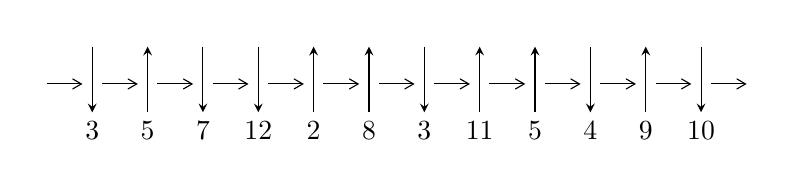
\begin{tikzpicture}[x=20pt, y=17pt]
	% nodes
	\node (C0) at (0, 0) {};
	\node (C1) at (1, 0) {};
	\node (C1U) at (1, +1) {};
	\node (C1D) at (1, -1) {3};

	\node (C2) at (2, 0) {};
	\node (C2U) at (2, +1) {};
	\node (C2D) at (2, -1) {5};

	\node (C3) at (3, 0) {};
	\node (C3U) at (3, +1) {};
	\node (C3D) at (3, -1) {7};

	\node (C4) at (4, 0) {};
	\node (C4U) at (4, +1) {};
	\node (C4D) at (4, -1) {12};

	\node (C5) at (5, 0) {};
	\node (C5U) at (5, +1) {};
	\node (C5D) at (5, -1) {2};

	\node (C6) at (6, 0) {};
	\node (C6U) at (6, +1) {};
	\node (C6D) at (6, -1) {8};

	\node (C7) at (7, 0) {};
	\node (C7U) at (7, +1) {};
	\node (C7D) at (7, -1) {3};

	\node (C8) at (8, 0) {};
	\node (C8U) at (8, +1) {};
	\node (C8D) at (8, -1) {11};

	\node (C9) at (9, 0) {};
	\node (C9U) at (9, +1) {};
	\node (C9D) at (9, -1) {5};

	\node (C10) at (10, 0) {};
	\node (C10U) at (10, +1) {};
	\node (C10D) at (10, -1) {4};

	\node (C11) at (11, 0) {};
	\node (C11U) at (11, +1) {};
	\node (C11D) at (11, -1) {9};

	\node (C12) at (12, 0) {};
	\node (C12U) at (12, +1) {};
	\node (C12D) at (12, -1) {10};
	\node (C13) at (13, 0) {};

	% arrows
	\draw[->,>={angle 60}]
	(C0) edge (C1) (C1) edge (C2) (C2) edge (C3) (C3) edge (C4) (C4) edge (C5) (C5) edge (C6) (C6) edge (C7) (C7) edge (C8) (C8) edge (C9) (C9) edge (C10) (C10) edge (C11) (C11) edge (C12) (C12) edge (C13) ;	\draw[->,>=stealth]
	(C1U) edge (C1D) (C2D) edge (C2U) (C3U) edge (C3D) (C4U) edge (C4D) (C5D) edge (C5U) (C6D) edge (C6U) (C7U) edge (C7D) (C8D) edge (C8U) (C9D) edge (C9U) (C10U) edge (C10D) (C11D) edge (C11U) (C12U) edge (C12D) ;
	\end{tikzpicture} \\
\hhline{~~} \\& 
\textbf{Solving Sequence} \\ \cline{2-2} 
 &
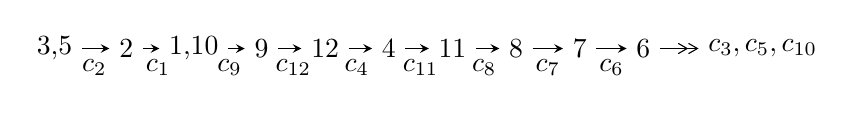
\begin{tikzpicture}[x=23pt, y=7pt]
	% node
	\node (A0) at (-1/8, 0) {3,5};
	\node (A1) at (1, 0) {2};
	\node (A2) at (33/16, 0) {1,10};
	\node (A3) at (25/8, 0) {9};
	\node (A4) at (33/8, 0) {12};
	\node (A5) at (41/8, 0) {4};
	\node (A6) at (49/8, 0) {11};
	\node (A7) at (57/8, 0) {8};
	\node (A8) at (65/8, 0) {7};
	\node (A9) at (73/8, 0) {6};
	\node (C1) at (1/2, -1) {$c_{2}$};
	\node (C2) at (3/2, -1) {$c_{1}$};
	\node (C3) at (21/8, -1) {$c_{9}$};
	\node (C4) at (29/8, -1) {$c_{12}$};
	\node (C5) at (37/8, -1) {$c_{4}$};
	\node (C6) at (45/8, -1) {$c_{11}$};
	\node (C7) at (53/8, -1) {$c_{8}$};
	\node (C8) at (61/8, -1) {$c_{7}$};
	\node (C9) at (69/8, -1) {$c_{6}$};
	\node (A10) at (11, 0) {$c_{3},c_{5},c_{10}$};

	% edge
	\draw[->,>=stealth]	
	(A0) edge (A1) (A1) edge (A2) (A2) edge (A3) (A3) edge (A4) (A4) edge (A5) (A5) edge (A6) (A6) edge (A7) (A7) edge (A8) (A8) edge (A9) ;
	\draw[->>,>={angle 60}]	
	(A9) edge (A10);
\end{tikzpicture} \\ 

\end{tabular} \\

\footnotetext{
The image of knot diagram is generated by the software ``\textbf{Draw programme}" developed by Andrew Bartholomew(\url{http://www.layer8.co.uk/maths/draw/index.htm\#Running-draw}), where we modified some parts for our purpose(\url{https://github.com/CATsTAILs/LinksPainter}).
}\phantom \\ \newline 
\centering \textbf{Ideals for irreducible components\footnotemark of $X_{\text{par}}$} 
 
\begin{align*}
I^u_{1}&=\langle 
6.94451\times10^{73} u^{53}-1.34116\times10^{74} u^{52}+\cdots+3.81141\times10^{75} b-1.25088\times10^{75},\\
\phantom{I^u_{1}}&\phantom{= \langle  }-3.43142\times10^{75} u^{53}+7.05210\times10^{75} u^{52}+\cdots+3.23970\times10^{76} a+1.89860\times10^{77},\\
\phantom{I^u_{1}}&\phantom{= \langle  }u^{54}-2 u^{53}+\cdots-112 u+17\rangle \\
I^u_{2}&=\langle 
-44 u^{17}+4 u^{16}+\cdots+69 b+127 u,\;-44 u^{17}-264 u^{15}+\cdots+69 a-224,\;u^{18}+6 u^{16}+\cdots+3 u+1\rangle \\
I^u_{3}&=\langle 
a^4- a^3 u+2 a^2- a u+b- u+2,\;a^5- a^4+2 a^3- a^2+a-1,\;u^2+1\rangle \\
I^u_{4}&=\langle 
-3 u^3+6 u^2+4 b-5 u+1,\;u^3+2 a- u+3,\;u^4- u^3+u^2+1\rangle \\
\\
\end{align*}
\raggedright * 4 irreducible components of $\dim_{\mathbb{C}}=0$, with total 86 representations.\\
\footnotetext{All coefficients of polynomials are rational numbers. But the coefficients are sometimes approximated in decimal forms when there is not enough margin.}
\newpage
\renewcommand{\arraystretch}{1}
\centering \section*{I. $I^u_{1}= \langle 6.94\times10^{73} u^{53}-1.34\times10^{74} u^{52}+\cdots+3.81\times10^{75} b-1.25\times10^{75},\;-3.43\times10^{75} u^{53}+7.05\times10^{75} u^{52}+\cdots+3.24\times10^{76} a+1.90\times10^{77},\;u^{54}-2 u^{53}+\cdots-112 u+17 \rangle$}
\flushleft \textbf{(i) Arc colorings}\\
\begin{tabular}{m{7pt} m{180pt} m{7pt} m{180pt} }
\flushright $a_{3}=$&$\begin{pmatrix}1\\0\end{pmatrix}$ \\
\flushright $a_{5}=$&$\begin{pmatrix}0\\u\end{pmatrix}$ \\
\flushright $a_{2}=$&$\begin{pmatrix}1\\u^2\end{pmatrix}$ \\
\flushright $a_{1}=$&$\begin{pmatrix}u^2+1\\u^2\end{pmatrix}$ \\
\flushright $a_{10}=$&$\begin{pmatrix}0.105918 u^{53}-0.217677 u^{52}+\cdots+63.2432 u-5.86042\\-0.0182203 u^{53}+0.0351879 u^{52}+\cdots-10.1732 u+0.328192\end{pmatrix}$ \\
\flushright $a_{9}=$&$\begin{pmatrix}0.105918 u^{53}-0.217677 u^{52}+\cdots+63.2432 u-5.86042\\-0.0293505 u^{53}+0.0578164 u^{52}+\cdots-12.6281 u+0.427504\end{pmatrix}$ \\
\flushright $a_{12}=$&$\begin{pmatrix}-0.0377580 u^{53}+0.0561954 u^{52}+\cdots+17.7971 u-6.35371\\-0.0210496 u^{53}+0.0288416 u^{52}+\cdots-9.16703 u+1.99686\end{pmatrix}$ \\
\flushright $a_{4}=$&$\begin{pmatrix}0.0736388 u^{53}-0.109834 u^{52}+\cdots+5.97498 u+3.87914\\-0.00164042 u^{53}+0.00683312 u^{52}+\cdots-1.67223 u-0.577146\end{pmatrix}$ \\
\flushright $a_{11}=$&$\begin{pmatrix}0.0157800 u^{53}-0.0231466 u^{52}+\cdots+29.3692 u-3.16089\\-0.0328608 u^{53}+0.0646084 u^{52}+\cdots-11.4634 u+0.980987\end{pmatrix}$ \\
\flushright $a_{8}=$&$\begin{pmatrix}0.0000582809 u^{53}+0.00965479 u^{52}+\cdots+26.4948 u-4.19485\\-0.0248738 u^{53}+0.0481071 u^{52}+\cdots-11.7942 u+1.11363\end{pmatrix}$ \\
\flushright $a_{7}=$&$\begin{pmatrix}-0.0248155 u^{53}+0.0577619 u^{52}+\cdots+14.7006 u-3.08122\\-0.0248738 u^{53}+0.0481071 u^{52}+\cdots-11.7942 u+1.11363\end{pmatrix}$ \\
\flushright $a_{6}=$&$\begin{pmatrix}- u\\- u^3- u\end{pmatrix}$\\&\end{tabular}
\flushleft \textbf{(ii) Obstruction class $= -1$}\\~\\
\flushleft \textbf{(iii) Cusp Shapes $= 0.0961909 u^{53}-0.214297 u^{52}+\cdots+61.1959 u+0.495059$}\\~\\
\newpage\renewcommand{\arraystretch}{1}
\flushleft \textbf{(iv) u-Polynomials at the component}\newline \\
\begin{tabular}{m{50pt}|m{274pt}}
Crossings & \hspace{64pt}u-Polynomials at each crossing \\
\hline $$\begin{aligned}c_{1}\end{aligned}$$&$\begin{aligned}
&u^{54}+60 u^{53}+\cdots+17614 u+289
\end{aligned}$\\
\hline $$\begin{aligned}c_{2},c_{5}\end{aligned}$$&$\begin{aligned}
&u^{54}+2 u^{53}+\cdots+112 u+17
\end{aligned}$\\
\hline $$\begin{aligned}c_{3},c_{7}\end{aligned}$$&$\begin{aligned}
&u^{54}+2 u^{53}+\cdots+20 u+17
\end{aligned}$\\
\hline $$\begin{aligned}c_{4}\end{aligned}$$&$\begin{aligned}
&u^{54}-7 u^{53}+\cdots-8 u+4
\end{aligned}$\\
\hline $$\begin{aligned}c_{6}\end{aligned}$$&$\begin{aligned}
&u^{54}-20 u^{53}+\cdots-15886 u+289
\end{aligned}$\\
\hline $$\begin{aligned}c_{8},c_{11}\end{aligned}$$&$\begin{aligned}
&u^{54}+4 u^{53}+\cdots+481 u+16
\end{aligned}$\\
\hline $$\begin{aligned}c_{9}\end{aligned}$$&$\begin{aligned}
&2(2 u^{54}+11 u^{53}+\cdots+27633 u+3982)
\end{aligned}$\\
\hline $$\begin{aligned}c_{10}\end{aligned}$$&$\begin{aligned}
&2(2 u^{54}+3 u^{53}+\cdots-26787 u+17894)
\end{aligned}$\\
\hline $$\begin{aligned}c_{12}\end{aligned}$$&$\begin{aligned}
&u^{54}-8 u^{53}+\cdots-2976 u+256
\end{aligned}$\\
\hline
\end{tabular}\\~\\
\newpage\renewcommand{\arraystretch}{1}
\flushleft \textbf{(v) Riley Polynomials at the component}\newline \\
\begin{tabular}{m{50pt}|m{274pt}}
Crossings & \hspace{64pt}Riley Polynomials at each crossing \\
\hline $$\begin{aligned}c_{1}\end{aligned}$$&$\begin{aligned}
&y^{54}-120 y^{53}+\cdots-34842354 y+83521
\end{aligned}$\\
\hline $$\begin{aligned}c_{2},c_{5}\end{aligned}$$&$\begin{aligned}
&y^{54}+60 y^{53}+\cdots+17614 y+289
\end{aligned}$\\
\hline $$\begin{aligned}c_{3},c_{7}\end{aligned}$$&$\begin{aligned}
&y^{54}+20 y^{53}+\cdots+15886 y+289
\end{aligned}$\\
\hline $$\begin{aligned}c_{4}\end{aligned}$$&$\begin{aligned}
&y^{54}+17 y^{53}+\cdots+152 y+16
\end{aligned}$\\
\hline $$\begin{aligned}c_{6}\end{aligned}$$&$\begin{aligned}
&y^{54}+40 y^{53}+\cdots-35600546 y+83521
\end{aligned}$\\
\hline $$\begin{aligned}c_{8},c_{11}\end{aligned}$$&$\begin{aligned}
&y^{54}-32 y^{53}+\cdots-95457 y+256
\end{aligned}$\\
\hline $$\begin{aligned}c_{9}\end{aligned}$$&$\begin{aligned}
&4(4 y^{54}-173 y^{53}+\cdots+1.70212\times10^{8} y+1.58563\times10^{7})
\end{aligned}$\\
\hline $$\begin{aligned}c_{10}\end{aligned}$$&$\begin{aligned}
&4(4 y^{54}-205 y^{53}+\cdots+5.53025\times10^{9} y+3.20195\times10^{8})
\end{aligned}$\\
\hline $$\begin{aligned}c_{12}\end{aligned}$$&$\begin{aligned}
&y^{54}-12 y^{53}+\cdots-1545216 y+65536
\end{aligned}$\\
\hline
\end{tabular}\\~\\
\newpage\flushleft \textbf{(vi) Complex Volumes and Cusp Shapes}
$$\begin{array}{c|c|c}  
\text{Solutions to }I^u_{1}& \I (\text{vol} + \sqrt{-1}CS) & \text{Cusp shape}\\
 \hline 
\begin{aligned}
u &= -0.957433 + 0.281564 I \\
a &= -0.366782 + 0.368685 I \\
b &= -0.536027 - 0.041780 I\end{aligned}
 & \phantom{-}0.08167 - 4.27758 I & \phantom{-0.000000 -}0. + 6.47467 I \\ \hline\begin{aligned}
u &= -0.957433 - 0.281564 I \\
a &= -0.366782 - 0.368685 I \\
b &= -0.536027 + 0.041780 I\end{aligned}
 & \phantom{-}0.08167 + 4.27758 I & \phantom{-0.000000 } 0. - 6.47467 I \\ \hline\begin{aligned}
u &= \phantom{-}0.793853 + 0.517771 I \\
a &= -0.989605 - 0.419229 I \\
b &= -0.745351 + 0.352281 I\end{aligned}
 & -1.69843 + 5.87991 I & -0.83203 - 7.69197 I \\ \hline\begin{aligned}
u &= \phantom{-}0.793853 - 0.517771 I \\
a &= -0.989605 + 0.419229 I \\
b &= -0.745351 - 0.352281 I\end{aligned}
 & -1.69843 - 5.87991 I & -0.83203 + 7.69197 I \\ \hline\begin{aligned}
u &= \phantom{-}1.013690 + 0.409819 I \\
a &= \phantom{-}1.40509 + 0.61654 I \\
b &= \phantom{-}1.023680 - 0.012588 I\end{aligned}
 & \phantom{-}1.51017 + 11.89510 I & \phantom{-0.000000 } 0. - 8.55352 I \\ \hline\begin{aligned}
u &= \phantom{-}1.013690 - 0.409819 I \\
a &= \phantom{-}1.40509 - 0.61654 I \\
b &= \phantom{-}1.023680 + 0.012588 I\end{aligned}
 & \phantom{-}1.51017 - 11.89510 I & \phantom{-0.000000 -}0. + 8.55352 I \\ \hline\begin{aligned}
u &= \phantom{-}0.037687 + 0.876774 I \\
a &= -0.411613 - 0.841558 I \\
b &= -0.730721 - 0.454623 I\end{aligned}
 & -1.21558 - 1.50306 I & -6.28567 + 3.87694 I \\ \hline\begin{aligned}
u &= \phantom{-}0.037687 - 0.876774 I \\
a &= -0.411613 + 0.841558 I \\
b &= -0.730721 + 0.454623 I\end{aligned}
 & -1.21558 + 1.50306 I & -6.28567 - 3.87694 I \\ \hline\begin{aligned}
u &= \phantom{-}0.001197 + 1.155080 I \\
a &= \phantom{-}0.344466 + 1.134660 I \\
b &= \phantom{-}0.086158 + 0.503268 I\end{aligned}
 & \phantom{-}4.74660 - 4.32144 I & \phantom{-0.000000 } 0 \\ \hline\begin{aligned}
u &= \phantom{-}0.001197 - 1.155080 I \\
a &= \phantom{-}0.344466 - 1.134660 I \\
b &= \phantom{-}0.086158 - 0.503268 I\end{aligned}
 & \phantom{-}4.74660 + 4.32144 I & \phantom{-0.000000 } 0\\
 \hline 
 \end{array}$$\newpage$$\begin{array}{c|c|c}  
\text{Solutions to }I^u_{1}& \I (\text{vol} + \sqrt{-1}CS) & \text{Cusp shape}\\
 \hline 
\begin{aligned}
u &= -0.904014 + 0.749313 I \\
a &= \phantom{-}0.409227 - 0.949421 I \\
b &= \phantom{-}0.254579 - 0.478630 I\end{aligned}
 & -0.351082 - 0.581835 I & \phantom{-0.000000 } 0 \\ \hline\begin{aligned}
u &= -0.904014 - 0.749313 I \\
a &= \phantom{-}0.409227 + 0.949421 I \\
b &= \phantom{-}0.254579 + 0.478630 I\end{aligned}
 & -0.351082 + 0.581835 I & \phantom{-0.000000 } 0 \\ \hline\begin{aligned}
u &= -0.409754 + 0.654267 I \\
a &= \phantom{-}0.670688 - 0.470147 I \\
b &= \phantom{-}0.024664 - 0.332222 I\end{aligned}
 & -0.11724 - 1.46636 I & -1.51920 + 4.74355 I \\ \hline\begin{aligned}
u &= -0.409754 - 0.654267 I \\
a &= \phantom{-}0.670688 + 0.470147 I \\
b &= \phantom{-}0.024664 + 0.332222 I\end{aligned}
 & -0.11724 + 1.46636 I & -1.51920 - 4.74355 I \\ \hline\begin{aligned}
u &= \phantom{-}0.897207 + 0.878746 I \\
a &= \phantom{-}0.412964 + 0.196074 I \\
b &= \phantom{-}0.230506 + 0.127637 I\end{aligned}
 & \phantom{-}8.36051 + 3.29219 I & \phantom{-0.000000 } 0 \\ \hline\begin{aligned}
u &= \phantom{-}0.897207 - 0.878746 I \\
a &= \phantom{-}0.412964 - 0.196074 I \\
b &= \phantom{-}0.230506 - 0.127637 I\end{aligned}
 & \phantom{-}8.36051 - 3.29219 I & \phantom{-0.000000 } 0 \\ \hline\begin{aligned}
u &= \phantom{-}0.611149 + 0.347151 I \\
a &= \phantom{-}1.350850 - 0.353105 I \\
b &= \phantom{-}1.28376 + 1.02238 I\end{aligned}
 & \phantom{-}3.32384 + 4.22762 I & \phantom{-}7.57484 - 8.95989 I \\ \hline\begin{aligned}
u &= \phantom{-}0.611149 - 0.347151 I \\
a &= \phantom{-}1.350850 + 0.353105 I \\
b &= \phantom{-}1.28376 - 1.02238 I\end{aligned}
 & \phantom{-}3.32384 - 4.22762 I & \phantom{-}7.57484 + 8.95989 I \\ \hline\begin{aligned}
u &= -0.483135 + 0.456682 I \\
a &= -2.56114 - 3.18734 I \\
b &= -1.88415 + 0.56985 I\end{aligned}
 & \phantom{-}1.86209 - 1.74879 I & \phantom{-}7.3853 - 15.6719 I \\ \hline\begin{aligned}
u &= -0.483135 - 0.456682 I \\
a &= -2.56114 + 3.18734 I \\
b &= -1.88415 - 0.56985 I\end{aligned}
 & \phantom{-}1.86209 + 1.74879 I & \phantom{-}7.3853 + 15.6719 I\\
 \hline 
 \end{array}$$\newpage$$\begin{array}{c|c|c}  
\text{Solutions to }I^u_{1}& \I (\text{vol} + \sqrt{-1}CS) & \text{Cusp shape}\\
 \hline 
\begin{aligned}
u &= -0.246711 + 0.521269 I \\
a &= \phantom{-}2.52817 + 2.38441 I \\
b &= \phantom{-}0.71366 - 1.77517 I\end{aligned}
 & \phantom{-}1.60277 - 1.13073 I & \phantom{-}16.4890 + 3.6045 I \\ \hline\begin{aligned}
u &= -0.246711 - 0.521269 I \\
a &= \phantom{-}2.52817 - 2.38441 I \\
b &= \phantom{-}0.71366 + 1.77517 I\end{aligned}
 & \phantom{-}1.60277 + 1.13073 I & \phantom{-}16.4890 - 3.6045 I \\ \hline\begin{aligned}
u &= \phantom{-}0.10747 + 1.43757 I \\
a &= -0.231658 + 0.116000 I \\
b &= -2.40283 - 0.09567 I\end{aligned}
 & -1.12918 + 2.68232 I & \phantom{-0.000000 } 0 \\ \hline\begin{aligned}
u &= \phantom{-}0.10747 - 1.43757 I \\
a &= -0.231658 - 0.116000 I \\
b &= -2.40283 + 0.09567 I\end{aligned}
 & -1.12918 - 2.68232 I & \phantom{-0.000000 } 0 \\ \hline\begin{aligned}
u &= -0.00780 + 1.45535 I \\
a &= -0.234240 - 0.821894 I \\
b &= -0.634589 + 0.224881 I\end{aligned}
 & -3.51163 - 1.45830 I & \phantom{-0.000000 } 0 \\ \hline\begin{aligned}
u &= -0.00780 - 1.45535 I \\
a &= -0.234240 + 0.821894 I \\
b &= -0.634589 - 0.224881 I\end{aligned}
 & -3.51163 + 1.45830 I & \phantom{-0.000000 } 0 \\ \hline\begin{aligned}
u &= \phantom{-}0.19633 + 1.47266 I \\
a &= -0.180761 + 0.764063 I \\
b &= -0.450752 - 0.458790 I\end{aligned}
 & -2.64331 + 7.12189 I & \phantom{-0.000000 } 0 \\ \hline\begin{aligned}
u &= \phantom{-}0.19633 - 1.47266 I \\
a &= -0.180761 - 0.764063 I \\
b &= -0.450752 + 0.458790 I\end{aligned}
 & -2.64331 - 7.12189 I & \phantom{-0.000000 } 0 \\ \hline\begin{aligned}
u &= -0.04819 + 1.51041 I \\
a &= \phantom{-}0.39189 - 1.67295 I \\
b &= \phantom{-}0.87803 - 2.40931 I\end{aligned}
 & -5.05765 - 2.00436 I & \phantom{-0.000000 } 0 \\ \hline\begin{aligned}
u &= -0.04819 - 1.51041 I \\
a &= \phantom{-}0.39189 + 1.67295 I \\
b &= \phantom{-}0.87803 + 2.40931 I\end{aligned}
 & -5.05765 + 2.00436 I & \phantom{-0.000000 } 0\\
 \hline 
 \end{array}$$\newpage$$\begin{array}{c|c|c}  
\text{Solutions to }I^u_{1}& \I (\text{vol} + \sqrt{-1}CS) & \text{Cusp shape}\\
 \hline 
\begin{aligned}
u &= -0.14469 + 1.50993 I \\
a &= \phantom{-}0.47360 + 1.91984 I \\
b &= \phantom{-}1.53856 + 2.59401 I\end{aligned}
 & -4.66611 - 3.99543 I & \phantom{-0.000000 } 0 \\ \hline\begin{aligned}
u &= -0.14469 - 1.50993 I \\
a &= \phantom{-}0.47360 - 1.91984 I \\
b &= \phantom{-}1.53856 - 2.59401 I\end{aligned}
 & -4.66611 + 3.99543 I & \phantom{-0.000000 } 0 \\ \hline\begin{aligned}
u &= \phantom{-}0.416507 + 0.239610 I \\
a &= \phantom{-}0.373760 - 0.682809 I \\
b &= \phantom{-}1.212780 - 0.597298 I\end{aligned}
 & \phantom{-}4.35238 + 0.88122 I & \phantom{-}11.36984 - 2.33709 I \\ \hline\begin{aligned}
u &= \phantom{-}0.416507 - 0.239610 I \\
a &= \phantom{-}0.373760 + 0.682809 I \\
b &= \phantom{-}1.212780 + 0.597298 I\end{aligned}
 & \phantom{-}4.35238 - 0.88122 I & \phantom{-}11.36984 + 2.33709 I \\ \hline\begin{aligned}
u &= \phantom{-}0.076348 + 0.449359 I \\
a &= \phantom{-}1.54451 - 2.17798 I \\
b &= \phantom{-}0.371098 - 0.688121 I\end{aligned}
 & \phantom{-}7.12845 + 4.50045 I & \phantom{-}11.43251 - 4.54345 I \\ \hline\begin{aligned}
u &= \phantom{-}0.076348 - 0.449359 I \\
a &= \phantom{-}1.54451 + 2.17798 I \\
b &= \phantom{-}0.371098 + 0.688121 I\end{aligned}
 & \phantom{-}7.12845 - 4.50045 I & \phantom{-}11.43251 + 4.54345 I \\ \hline\begin{aligned}
u &= -0.40434 + 1.49345 I \\
a &= \phantom{-}0.473577 + 0.252036 I \\
b &= \phantom{-}1.54220 - 0.04301 I\end{aligned}
 & -5.61605 - 9.26553 I & \phantom{-0.000000 } 0 \\ \hline\begin{aligned}
u &= -0.40434 - 1.49345 I \\
a &= \phantom{-}0.473577 - 0.252036 I \\
b &= \phantom{-}1.54220 + 0.04301 I\end{aligned}
 & -5.61605 + 9.26553 I & \phantom{-0.000000 } 0 \\ \hline\begin{aligned}
u &= \phantom{-}0.30238 + 1.53005 I \\
a &= \phantom{-}0.508036 - 0.093774 I \\
b &= \phantom{-}1.60740 + 0.32922 I\end{aligned}
 & -8.31392 + 2.90879 I & \phantom{-0.000000 } 0 \\ \hline\begin{aligned}
u &= \phantom{-}0.30238 - 1.53005 I \\
a &= \phantom{-}0.508036 + 0.093774 I \\
b &= \phantom{-}1.60740 - 0.32922 I\end{aligned}
 & -8.31392 - 2.90879 I & \phantom{-0.000000 } 0\\
 \hline 
 \end{array}$$\newpage$$\begin{array}{c|c|c}  
\text{Solutions to }I^u_{1}& \I (\text{vol} + \sqrt{-1}CS) & \text{Cusp shape}\\
 \hline 
\begin{aligned}
u &= \phantom{-}0.27909 + 1.54859 I \\
a &= \phantom{-}0.761075 - 0.328934 I \\
b &= \phantom{-}2.56556 - 0.27826 I\end{aligned}
 & -8.47521 + 9.84153 I & \phantom{-0.000000 } 0 \\ \hline\begin{aligned}
u &= \phantom{-}0.27909 - 1.54859 I \\
a &= \phantom{-}0.761075 + 0.328934 I \\
b &= \phantom{-}2.56556 + 0.27826 I\end{aligned}
 & -8.47521 - 9.84153 I & \phantom{-0.000000 } 0 \\ \hline\begin{aligned}
u &= \phantom{-}0.39619 + 1.53466 I \\
a &= -0.989911 + 0.661170 I \\
b &= -2.69175 + 0.38369 I\end{aligned}
 & -4.7262 + 17.0140 I & \phantom{-0.000000 } 0 \\ \hline\begin{aligned}
u &= \phantom{-}0.39619 - 1.53466 I \\
a &= -0.989911 - 0.661170 I \\
b &= -2.69175 - 0.38369 I\end{aligned}
 & -4.7262 - 17.0140 I & \phantom{-0.000000 } 0 \\ \hline\begin{aligned}
u &= -0.13238 + 1.58588 I \\
a &= \phantom{-}0.710747 + 0.251585 I \\
b &= \phantom{-}2.39257 + 0.46175 I\end{aligned}
 & -10.02230 - 3.29278 I & \phantom{-0.000000 } 0 \\ \hline\begin{aligned}
u &= -0.13238 - 1.58588 I \\
a &= \phantom{-}0.710747 - 0.251585 I \\
b &= \phantom{-}2.39257 - 0.46175 I\end{aligned}
 & -10.02230 + 3.29278 I & \phantom{-0.000000 } 0 \\ \hline\begin{aligned}
u &= -0.23845 + 1.60519 I \\
a &= -1.019030 - 0.001725 I \\
b &= -2.17248 + 0.26878 I\end{aligned}
 & -8.27340 - 4.54754 I & \phantom{-0.000000 } 0 \\ \hline\begin{aligned}
u &= -0.23845 - 1.60519 I \\
a &= -1.019030 + 0.001725 I \\
b &= -2.17248 - 0.26878 I\end{aligned}
 & -8.27340 + 4.54754 I & \phantom{-0.000000 } 0 \\ \hline\begin{aligned}
u &= -0.30330 + 1.60247 I \\
a &= -0.977488 - 0.584250 I \\
b &= -2.55816 - 0.50781 I\end{aligned}
 & -7.29392 - 10.27410 I & \phantom{-0.000000 } 0 \\ \hline\begin{aligned}
u &= -0.30330 - 1.60247 I \\
a &= -0.977488 + 0.584250 I \\
b &= -2.55816 + 0.50781 I\end{aligned}
 & -7.29392 + 10.27410 I & \phantom{-0.000000 } 0\\
 \hline 
 \end{array}$$\newpage$$\begin{array}{c|c|c}  
\text{Solutions to }I^u_{1}& \I (\text{vol} + \sqrt{-1}CS) & \text{Cusp shape}\\
 \hline 
\begin{aligned}
u &= \phantom{-}0.09043 + 1.66784 I \\
a &= -0.977056 - 0.182021 I \\
b &= -2.14804 - 0.39830 I\end{aligned}
 & -9.44818 - 2.46020 I & \phantom{-0.000000 } 0 \\ \hline\begin{aligned}
u &= \phantom{-}0.09043 - 1.66784 I \\
a &= -0.977056 + 0.182021 I \\
b &= -2.14804 + 0.39830 I\end{aligned}
 & -9.44818 + 2.46020 I & \phantom{-0.000000 } 0 \\ \hline\begin{aligned}
u &= \phantom{-}0.060670 + 0.183744 I \\
a &= \phantom{-}0.36004 + 5.05217 I \\
b &= -0.395346 - 1.125760 I\end{aligned}
 & \phantom{-}1.88776 - 1.50114 I & \phantom{-}7.21238 + 4.30156 I \\ \hline\begin{aligned}
u &= \phantom{-}0.060670 - 0.183744 I \\
a &= \phantom{-}0.36004 - 5.05217 I \\
b &= -0.395346 + 1.125760 I\end{aligned}
 & \phantom{-}1.88776 + 1.50114 I & \phantom{-}7.21238 - 4.30156 I\\
 \hline 
 \end{array}$$\newpage\newpage\renewcommand{\arraystretch}{1}
\centering \section*{II. $I^u_{2}= \langle -44 u^{17}+4 u^{16}+\cdots+69 b+127 u,\;-44 u^{17}-264 u^{15}+\cdots+69 a-224,\;u^{18}+6 u^{16}+\cdots+3 u+1 \rangle$}
\flushleft \textbf{(i) Arc colorings}\\
\begin{tabular}{m{7pt} m{180pt} m{7pt} m{180pt} }
\flushright $a_{3}=$&$\begin{pmatrix}1\\0\end{pmatrix}$ \\
\flushright $a_{5}=$&$\begin{pmatrix}0\\u\end{pmatrix}$ \\
\flushright $a_{2}=$&$\begin{pmatrix}1\\u^2\end{pmatrix}$ \\
\flushright $a_{1}=$&$\begin{pmatrix}u^2+1\\u^2\end{pmatrix}$ \\
\flushright $a_{10}=$&$\begin{pmatrix}0.637681 u^{17}+3.82609 u^{15}+\cdots+2.66667 u+3.24638\\0.637681 u^{17}-0.0579710 u^{16}+\cdots+3.91304 u^{2}-1.84058 u\end{pmatrix}$ \\
\flushright $a_{9}=$&$\begin{pmatrix}0.637681 u^{17}+3.82609 u^{15}+\cdots+2.66667 u+3.24638\\0.637681 u^{17}+0.173913 u^{16}+\cdots+5.24638 u^{2}-2.47826 u\end{pmatrix}$ \\
\flushright $a_{12}=$&$\begin{pmatrix}0.594203 u^{17}+3.56522 u^{15}+\cdots+3.66667 u+0.115942\\0.594203 u^{17}-0.594203 u^{16}+\cdots-3.55072 u^{2}-0.115942 u\end{pmatrix}$ \\
\flushright $a_{4}=$&$\begin{pmatrix}u^2+1\\u^2\end{pmatrix}$ \\
\flushright $a_{11}=$&$\begin{pmatrix}0.840580 u^{17}+5.04348 u^{15}+\cdots+4.33333 u+3.18841\\0.840580 u^{17}-0.0579710 u^{16}+\cdots+3.85507 u^{2}-1.84058 u\end{pmatrix}$ \\
\flushright $a_{8}=$&$\begin{pmatrix}0\\- u\end{pmatrix}$ \\
\flushright $a_{7}=$&$\begin{pmatrix}- u\\- u\end{pmatrix}$ \\
\flushright $a_{6}=$&$\begin{pmatrix}- u\\- u^3- u\end{pmatrix}$\\&\end{tabular}
\flushleft \textbf{(ii) Obstruction class $= -1$}\\~\\
\flushleft \textbf{(iii) Cusp Shapes $= \frac{20}{23} u^{15}+\frac{100}{23} u^{13}+\frac{44}{23} u^{12}+\frac{200}{23} u^{11}+\frac{176}{23} u^{10}+\frac{316}{23} u^9+\frac{264}{23} u^8+\frac{448}{23} u^7+\frac{260}{23} u^6+16 u^5+\frac{212}{23} u^4+\frac{208}{23} u^3+\frac{84}{23} u^2+4 u+\frac{106}{23}$}\\~\\
\newpage\renewcommand{\arraystretch}{1}
\flushleft \textbf{(iv) u-Polynomials at the component}\newline \\
\begin{tabular}{m{50pt}|m{274pt}}
Crossings & \hspace{64pt}u-Polynomials at each crossing \\
\hline $$\begin{aligned}c_{1}\end{aligned}$$&$\begin{aligned}
&u^{18}+12 u^{17}+\cdots+3 u+1
\end{aligned}$\\
\hline $$\begin{aligned}c_{2},c_{3},c_{5}\\c_{7}\end{aligned}$$&$\begin{aligned}
&u^{18}+6 u^{16}+\cdots-3 u+1
\end{aligned}$\\
\hline $$\begin{aligned}c_{4}\end{aligned}$$&$\begin{aligned}
&(u^6+3 u^5+5 u^4+4 u^3+2 u^2+u+1)^3
\end{aligned}$\\
\hline $$\begin{aligned}c_{6}\end{aligned}$$&$\begin{aligned}
&u^{18}-12 u^{17}+\cdots-3 u+1
\end{aligned}$\\
\hline $$\begin{aligned}c_{8},c_{11}\end{aligned}$$&$\begin{aligned}
&(u^6+u^5- u^4-2 u^3+u+1)^3
\end{aligned}$\\
\hline $$\begin{aligned}c_{9}\end{aligned}$$&$\begin{aligned}
&(u^6-3 u^5+5 u^4-4 u^3+2 u^2- u+1)^3
\end{aligned}$\\
\hline $$\begin{aligned}c_{10},c_{12}\end{aligned}$$&$\begin{aligned}
&(u^6- u^5- u^4+2 u^3- u+1)^3
\end{aligned}$\\
\hline
\end{tabular}\\~\\
\newpage\renewcommand{\arraystretch}{1}
\flushleft \textbf{(v) Riley Polynomials at the component}\newline \\
\begin{tabular}{m{50pt}|m{274pt}}
Crossings & \hspace{64pt}Riley Polynomials at each crossing \\
\hline $$\begin{aligned}c_{1},c_{6}\end{aligned}$$&$\begin{aligned}
&y^{18}-12 y^{17}+\cdots+95 y+1
\end{aligned}$\\
\hline $$\begin{aligned}c_{2},c_{3},c_{5}\\c_{7}\end{aligned}$$&$\begin{aligned}
&y^{18}+12 y^{17}+\cdots+3 y+1
\end{aligned}$\\
\hline $$\begin{aligned}c_{4},c_{9}\end{aligned}$$&$\begin{aligned}
&(y^6+y^5+5 y^4+6 y^2+3 y+1)^3
\end{aligned}$\\
\hline $$\begin{aligned}c_{8},c_{10},c_{11}\\c_{12}\end{aligned}$$&$\begin{aligned}
&(y^6-3 y^5+5 y^4-4 y^3+2 y^2- y+1)^3
\end{aligned}$\\
\hline
\end{tabular}\\~\\
\newpage\flushleft \textbf{(vi) Complex Volumes and Cusp Shapes}
$$\begin{array}{c|c|c}  
\text{Solutions to }I^u_{2}& \I (\text{vol} + \sqrt{-1}CS) & \text{Cusp shape}\\
 \hline 
\begin{aligned}
u &= -0.577722 + 0.852843 I \\
a &= -0.598036 + 0.102351 I \\
b &= -0.488236 - 0.375359 I\end{aligned}
 & -1.89061 - 0.92430 I & -3.71672 + 0.79423 I \\ \hline\begin{aligned}
u &= -0.577722 - 0.852843 I \\
a &= -0.598036 - 0.102351 I \\
b &= -0.488236 + 0.375359 I\end{aligned}
 & -1.89061 + 0.92430 I & -3.71672 - 0.79423 I \\ \hline\begin{aligned}
u &= \phantom{-}0.196160 + 0.885066 I \\
a &= \phantom{-}0.419078 + 1.129010 I \\
b &= -2.92263 - 1.35280 I\end{aligned}
 & \phantom{-}1.89061 - 0.92430 I & \phantom{-}3.71672 + 0.79423 I \\ \hline\begin{aligned}
u &= \phantom{-}0.196160 - 0.885066 I \\
a &= \phantom{-}0.419078 - 1.129010 I \\
b &= -2.92263 + 1.35280 I\end{aligned}
 & \phantom{-}1.89061 + 0.92430 I & \phantom{-}3.71672 - 0.79423 I \\ \hline\begin{aligned}
u &= -0.945163 + 0.610473 I \\
a &= \phantom{-}1.206700 - 0.490377 I \\
b &= \phantom{-}0.819070 - 0.094621 I\end{aligned}
 & \phantom{-0.000000 } -5.69302 I & \phantom{-0.000000 -}0. + 5.51057 I \\ \hline\begin{aligned}
u &= -0.945163 - 0.610473 I \\
a &= \phantom{-}1.206700 + 0.490377 I \\
b &= \phantom{-}0.819070 + 0.094621 I\end{aligned}
 & \phantom{-0.000000 -}5.69302 I & \phantom{-0.000000 } 0. - 5.51057 I \\ \hline\begin{aligned}
u &= \phantom{-}0.090472 + 1.133120 I \\
a &= -0.583686 + 0.762709 I \\
b &= -3.11733 - 0.76503 I\end{aligned}
 & \phantom{-}1.89061 + 0.92430 I & \phantom{-}3.71672 - 0.79423 I \\ \hline\begin{aligned}
u &= \phantom{-}0.090472 - 1.133120 I \\
a &= -0.583686 - 0.762709 I \\
b &= -3.11733 + 0.76503 I\end{aligned}
 & \phantom{-}1.89061 - 0.92430 I & \phantom{-}3.71672 + 0.79423 I \\ \hline\begin{aligned}
u &= \phantom{-}0.686633 + 0.502578 I \\
a &= -0.150201 - 0.718978 I \\
b &= -0.530542 - 0.156218 I\end{aligned}
 & -1.89061 - 0.92430 I & -3.71672 + 0.79423 I \\ \hline\begin{aligned}
u &= \phantom{-}0.686633 - 0.502578 I \\
a &= -0.150201 + 0.718978 I \\
b &= -0.530542 + 0.156218 I\end{aligned}
 & -1.89061 + 0.92430 I & -3.71672 - 0.79423 I\\
 \hline 
 \end{array}$$\newpage$$\begin{array}{c|c|c}  
\text{Solutions to }I^u_{2}& \I (\text{vol} + \sqrt{-1}CS) & \text{Cusp shape}\\
 \hline 
\begin{aligned}
u &= \phantom{-}0.824262 + 0.925280 I \\
a &= \phantom{-}0.271648 + 1.151080 I \\
b &= \phantom{-}0.190767 + 0.581448 I\end{aligned}
 & \phantom{-0.000000 } -5.69302 I & \phantom{-0.000000 -}0. + 5.51057 I \\ \hline\begin{aligned}
u &= \phantom{-}0.824262 - 0.925280 I \\
a &= \phantom{-}0.271648 - 1.151080 I \\
b &= \phantom{-}0.190767 - 0.581448 I\end{aligned}
 & \phantom{-0.000000 -}5.69302 I & \phantom{-0.000000 } 0. - 5.51057 I \\ \hline\begin{aligned}
u &= -0.108911 + 1.355420 I \\
a &= \phantom{-}0.402013 - 0.222804 I \\
b &= \phantom{-}1.71123 - 1.31922 I\end{aligned}
 & -1.89061 + 0.92430 I & -3.71672 - 0.79423 I \\ \hline\begin{aligned}
u &= -0.108911 - 1.355420 I \\
a &= \phantom{-}0.402013 + 0.222804 I \\
b &= \phantom{-}1.71123 + 1.31922 I\end{aligned}
 & -1.89061 - 0.92430 I & -3.71672 + 0.79423 I \\ \hline\begin{aligned}
u &= \phantom{-}0.12090 + 1.53575 I \\
a &= -0.819509 + 0.483205 I \\
b &= -2.32751 + 0.84183 I\end{aligned}
 & \phantom{-0.000000 -}5.69302 I & \phantom{-0.000000 } 0. - 5.51057 I \\ \hline\begin{aligned}
u &= \phantom{-}0.12090 - 1.53575 I \\
a &= -0.819509 - 0.483205 I \\
b &= -2.32751 - 0.84183 I\end{aligned}
 & \phantom{-0.000000 } -5.69302 I & \phantom{-0.000000 -}0. + 5.51057 I \\ \hline\begin{aligned}
u &= -0.286632 + 0.248050 I \\
a &= \phantom{-}2.85200 + 0.40141 I \\
b &= \phantom{-}0.665192 - 0.947661 I\end{aligned}
 & \phantom{-}1.89061 - 0.92430 I & \phantom{-}3.71672 + 0.79423 I \\ \hline\begin{aligned}
u &= -0.286632 - 0.248050 I \\
a &= \phantom{-}2.85200 - 0.40141 I \\
b &= \phantom{-}0.665192 + 0.947661 I\end{aligned}
 & \phantom{-}1.89061 + 0.92430 I & \phantom{-}3.71672 - 0.79423 I\\
 \hline 
 \end{array}$$\newpage\newpage\renewcommand{\arraystretch}{1}
\centering \section*{III. $I^u_{3}= \langle a^4- a^3 u+2 a^2- a u+b- u+2,\;a^5- a^4+2 a^3- a^2+a-1,\;u^2+1 \rangle$}
\flushleft \textbf{(i) Arc colorings}\\
\begin{tabular}{m{7pt} m{180pt} m{7pt} m{180pt} }
\flushright $a_{3}=$&$\begin{pmatrix}1\\0\end{pmatrix}$ \\
\flushright $a_{5}=$&$\begin{pmatrix}0\\u\end{pmatrix}$ \\
\flushright $a_{2}=$&$\begin{pmatrix}1\\-1\end{pmatrix}$ \\
\flushright $a_{1}=$&$\begin{pmatrix}0\\-1\end{pmatrix}$ \\
\flushright $a_{10}=$&$\begin{pmatrix}a\\- a^4+a^3 u-2 a^2+a u+u-2\end{pmatrix}$ \\
\flushright $a_{9}=$&$\begin{pmatrix}a\\- a^4+a^3 u-2 a^2+a u- a+u-2\end{pmatrix}$ \\
\flushright $a_{12}=$&$\begin{pmatrix}- a^2\\- a^4 u+a^4- a^2 u+a^2- a u+a\end{pmatrix}$ \\
\flushright $a_{4}=$&$\begin{pmatrix}a^4 u\\-1\end{pmatrix}$ \\
\flushright $a_{11}=$&$\begin{pmatrix}a^4\\- a^4-2 a^2+u-2\end{pmatrix}$ \\
\flushright $a_{8}=$&$\begin{pmatrix}a^4\\u\end{pmatrix}$ \\
\flushright $a_{7}=$&$\begin{pmatrix}a^4+u\\u\end{pmatrix}$ \\
\flushright $a_{6}=$&$\begin{pmatrix}u\\0\end{pmatrix}$\\&\end{tabular}
\flushleft \textbf{(ii) Obstruction class $= 1$}\\~\\
\flushleft \textbf{(iii) Cusp Shapes $= -4 a^3+4 a^2-4 a+4$}\\~\\
\newpage\renewcommand{\arraystretch}{1}
\flushleft \textbf{(iv) u-Polynomials at the component}\newline \\
\begin{tabular}{m{50pt}|m{274pt}}
Crossings & \hspace{64pt}u-Polynomials at each crossing \\
\hline $$\begin{aligned}c_{1}\end{aligned}$$&$\begin{aligned}
&(u-1)^{10}
\end{aligned}$\\
\hline $$\begin{aligned}c_{2},c_{3},c_{5}\\c_{7}\end{aligned}$$&$\begin{aligned}
&(u^2+1)^5
\end{aligned}$\\
\hline $$\begin{aligned}c_{4}\end{aligned}$$&$\begin{aligned}
&u^{10}+u^8+8 u^6+3 u^4+3 u^2+1
\end{aligned}$\\
\hline $$\begin{aligned}c_{6}\end{aligned}$$&$\begin{aligned}
&(u+1)^{10}
\end{aligned}$\\
\hline $$\begin{aligned}c_{8}\end{aligned}$$&$\begin{aligned}
&(u^5- u^4-2 u^3+u^2+u+1)^2
\end{aligned}$\\
\hline $$\begin{aligned}c_{9}\end{aligned}$$&$\begin{aligned}
&u^{10}-3 u^8+4 u^6- u^4- u^2+1
\end{aligned}$\\
\hline $$\begin{aligned}c_{10}\end{aligned}$$&$\begin{aligned}
&u^{10}+5 u^8+8 u^6+3 u^4- u^2+1
\end{aligned}$\\
\hline $$\begin{aligned}c_{11}\end{aligned}$$&$\begin{aligned}
&(u^5+u^4-2 u^3- u^2+u-1)^2
\end{aligned}$\\
\hline $$\begin{aligned}c_{12}\end{aligned}$$&$\begin{aligned}
&(u^5- u^4+2 u^3- u^2+u-1)^2
\end{aligned}$\\
\hline
\end{tabular}\\~\\
\newpage\renewcommand{\arraystretch}{1}
\flushleft \textbf{(v) Riley Polynomials at the component}\newline \\
\begin{tabular}{m{50pt}|m{274pt}}
Crossings & \hspace{64pt}Riley Polynomials at each crossing \\
\hline $$\begin{aligned}c_{1},c_{6}\end{aligned}$$&$\begin{aligned}
&(y-1)^{10}
\end{aligned}$\\
\hline $$\begin{aligned}c_{2},c_{3},c_{5}\\c_{7}\end{aligned}$$&$\begin{aligned}
&(y+1)^{10}
\end{aligned}$\\
\hline $$\begin{aligned}c_{4}\end{aligned}$$&$\begin{aligned}
&(y^5+y^4+8 y^3+3 y^2+3 y+1)^2
\end{aligned}$\\
\hline $$\begin{aligned}c_{8},c_{11}\end{aligned}$$&$\begin{aligned}
&(y^5-5 y^4+8 y^3-3 y^2- y-1)^2
\end{aligned}$\\
\hline $$\begin{aligned}c_{9}\end{aligned}$$&$\begin{aligned}
&(y^5-3 y^4+4 y^3- y^2- y+1)^2
\end{aligned}$\\
\hline $$\begin{aligned}c_{10}\end{aligned}$$&$\begin{aligned}
&(y^5+5 y^4+8 y^3+3 y^2- y+1)^2
\end{aligned}$\\
\hline $$\begin{aligned}c_{12}\end{aligned}$$&$\begin{aligned}
&(y^5+3 y^4+4 y^3+y^2- y-1)^2
\end{aligned}$\\
\hline
\end{tabular}\\~\\
\newpage\flushleft \textbf{(vi) Complex Volumes and Cusp Shapes}
$$\begin{array}{c|c|c}  
\text{Solutions to }I^u_{3}& \I (\text{vol} + \sqrt{-1}CS) & \text{Cusp shape}\\
 \hline 
\begin{aligned}
u &= \phantom{-0.000000 -}1.000000 I \\
a &= -0.339110 + 0.822375 I \\
b &= -1.43128 + 1.79928 I\end{aligned}
 & \phantom{-}0.32910 + 1.53058 I & \phantom{-}0.51511 - 4.43065 I \\ \hline\begin{aligned}
u &= \phantom{-0.000000 -}1.000000 I \\
a &= -0.339110 - 0.822375 I \\
b &= -0.331455 + 0.820551 I\end{aligned}
 & \phantom{-}0.32910 - 1.53058 I & \phantom{-}0.51511 + 4.43065 I \\ \hline\begin{aligned}
u &= \phantom{-0.000000 -}1.000000 I \\
a &= \phantom{-}0.766826\phantom{ +0.000000I} \\
b &= -3.52181 + 2.21774 I\end{aligned}
 & \phantom{-}2.40108\phantom{ +0.000000I} & \phantom{-}1.48110\phantom{ +0.000000I} \\ \hline\begin{aligned}
u &= \phantom{-0.000000 -}1.000000 I \\
a &= \phantom{-}0.455697 + 1.200150 I \\
b &= -0.0768928 + 0.0902877 I\end{aligned}
 & \phantom{-}5.87256 - 4.40083 I & \phantom{-}4.74431 + 3.49859 I \\ \hline\begin{aligned}
u &= \phantom{-0.000000 -}1.000000 I \\
a &= \phantom{-}0.455697 - 1.200150 I \\
b &= \phantom{-}0.361438 - 0.927855 I\end{aligned}
 & \phantom{-}5.87256 + 4.40083 I & \phantom{-}4.74431 - 3.49859 I \\ \hline\begin{aligned}
u &= \phantom{-0.000000 } -1.000000 I \\
a &= -0.339110 + 0.822375 I \\
b &= -0.331455 - 0.820551 I\end{aligned}
 & \phantom{-}0.32910 + 1.53058 I & \phantom{-}0.51511 - 4.43065 I \\ \hline\begin{aligned}
u &= \phantom{-0.000000 } -1.000000 I \\
a &= -0.339110 - 0.822375 I \\
b &= -1.43128 - 1.79928 I\end{aligned}
 & \phantom{-}0.32910 - 1.53058 I & \phantom{-}0.51511 + 4.43065 I \\ \hline\begin{aligned}
u &= \phantom{-0.000000 } -1.000000 I \\
a &= \phantom{-}0.766826\phantom{ +0.000000I} \\
b &= -3.52181 - 2.21774 I\end{aligned}
 & \phantom{-}2.40108\phantom{ +0.000000I} & \phantom{-}1.48110\phantom{ +0.000000I} \\ \hline\begin{aligned}
u &= \phantom{-0.000000 } -1.000000 I \\
a &= \phantom{-}0.455697 + 1.200150 I \\
b &= \phantom{-}0.361438 + 0.927855 I\end{aligned}
 & \phantom{-}5.87256 - 4.40083 I & \phantom{-}4.74431 + 3.49859 I \\ \hline\begin{aligned}
u &= \phantom{-0.000000 } -1.000000 I \\
a &= \phantom{-}0.455697 - 1.200150 I \\
b &= -0.0768928 - 0.0902877 I\end{aligned}
 & \phantom{-}5.87256 + 4.40083 I & \phantom{-}4.74431 - 3.49859 I\\
 \hline 
 \end{array}$$\newpage\newpage\renewcommand{\arraystretch}{1}
\centering \section*{IV. $I^u_{4}= \langle -3 u^3+6 u^2+4 b-5 u+1,\;u^3+2 a- u+3,\;u^4- u^3+u^2+1 \rangle$}
\flushleft \textbf{(i) Arc colorings}\\
\begin{tabular}{m{7pt} m{180pt} m{7pt} m{180pt} }
\flushright $a_{3}=$&$\begin{pmatrix}1\\0\end{pmatrix}$ \\
\flushright $a_{5}=$&$\begin{pmatrix}0\\u\end{pmatrix}$ \\
\flushright $a_{2}=$&$\begin{pmatrix}1\\u^2\end{pmatrix}$ \\
\flushright $a_{1}=$&$\begin{pmatrix}u^2+1\\u^2\end{pmatrix}$ \\
\flushright $a_{10}=$&$\begin{pmatrix}-\frac{1}{2} u^3+\frac{1}{2} u-\frac{3}{2}\\\frac{3}{4} u^3-\frac{3}{2} u^2+\frac{5}{4} u-\frac{1}{4}\end{pmatrix}$ \\
\flushright $a_{9}=$&$\begin{pmatrix}-\frac{1}{2} u^3+\frac{1}{2} u-\frac{3}{2}\\\frac{5}{4} u^3-\frac{5}{2} u^2+\frac{7}{4} u+\frac{1}{4}\end{pmatrix}$ \\
\flushright $a_{12}=$&$\begin{pmatrix}u^2+1\\u^2\end{pmatrix}$ \\
\flushright $a_{4}=$&$\begin{pmatrix}2 u^3- u^2-1\\u^3- u^2-1\end{pmatrix}$ \\
\flushright $a_{11}=$&$\begin{pmatrix}-\frac{1}{2} u^3+u^2+\frac{1}{2} u-\frac{1}{2}\\\frac{5}{4} u^3-\frac{3}{2} u^2+\frac{7}{4} u+\frac{1}{4}\end{pmatrix}$ \\
\flushright $a_{8}=$&$\begin{pmatrix}- u^2-1\\- u^2\end{pmatrix}$ \\
\flushright $a_{7}=$&$\begin{pmatrix}-2 u^2-1\\- u^2\end{pmatrix}$ \\
\flushright $a_{6}=$&$\begin{pmatrix}u\\u^3+u\end{pmatrix}$\\&\end{tabular}
\flushleft \textbf{(ii) Obstruction class $= 1$}\\~\\
\flushleft \textbf{(iii) Cusp Shapes $= \frac{71}{16} u^3+\frac{7}{8} u^2+\frac{241}{16} u+\frac{147}{16}$}\\~\\
\newpage\renewcommand{\arraystretch}{1}
\flushleft \textbf{(iv) u-Polynomials at the component}\newline \\
\begin{tabular}{m{50pt}|m{274pt}}
Crossings & \hspace{64pt}u-Polynomials at each crossing \\
\hline $$\begin{aligned}c_{1},c_{3}\end{aligned}$$&$\begin{aligned}
&u^4- u^3+3 u^2-2 u+1
\end{aligned}$\\
\hline $$\begin{aligned}c_{2}\end{aligned}$$&$\begin{aligned}
&u^4- u^3+u^2+1
\end{aligned}$\\
\hline $$\begin{aligned}c_{4}\end{aligned}$$&$\begin{aligned}
&u^4- u^3+5 u^2+u+2
\end{aligned}$\\
\hline $$\begin{aligned}c_{5}\end{aligned}$$&$\begin{aligned}
&u^4+u^3+u^2+1
\end{aligned}$\\
\hline $$\begin{aligned}c_{6}\end{aligned}$$&$\begin{aligned}
&u^4+5 u^3+7 u^2+2 u+1
\end{aligned}$\\
\hline $$\begin{aligned}c_{7}\end{aligned}$$&$\begin{aligned}
&u^4+u^3+3 u^2+2 u+1
\end{aligned}$\\
\hline $$\begin{aligned}c_{8}\end{aligned}$$&$\begin{aligned}
&(u+1)^4
\end{aligned}$\\
\hline $$\begin{aligned}c_{9},c_{10}\end{aligned}$$&$\begin{aligned}
&2(2 u^4- u^3+5 u^2+u+1)
\end{aligned}$\\
\hline $$\begin{aligned}c_{11}\end{aligned}$$&$\begin{aligned}
&(u-1)^4
\end{aligned}$\\
\hline $$\begin{aligned}c_{12}\end{aligned}$$&$\begin{aligned}
&u^4
\end{aligned}$\\
\hline
\end{tabular}\\~\\
\newpage\renewcommand{\arraystretch}{1}
\flushleft \textbf{(v) Riley Polynomials at the component}\newline \\
\begin{tabular}{m{50pt}|m{274pt}}
Crossings & \hspace{64pt}Riley Polynomials at each crossing \\
\hline $$\begin{aligned}c_{1},c_{3},c_{7}\end{aligned}$$&$\begin{aligned}
&y^4+5 y^3+7 y^2+2 y+1
\end{aligned}$\\
\hline $$\begin{aligned}c_{2},c_{5}\end{aligned}$$&$\begin{aligned}
&y^4+y^3+3 y^2+2 y+1
\end{aligned}$\\
\hline $$\begin{aligned}c_{4}\end{aligned}$$&$\begin{aligned}
&y^4+9 y^3+31 y^2+19 y+4
\end{aligned}$\\
\hline $$\begin{aligned}c_{6}\end{aligned}$$&$\begin{aligned}
&y^4-11 y^3+31 y^2+10 y+1
\end{aligned}$\\
\hline $$\begin{aligned}c_{8},c_{11}\end{aligned}$$&$\begin{aligned}
&(y-1)^4
\end{aligned}$\\
\hline $$\begin{aligned}c_{9},c_{10}\end{aligned}$$&$\begin{aligned}
&4(4 y^4+19 y^3+31 y^2+9 y+1)
\end{aligned}$\\
\hline $$\begin{aligned}c_{12}\end{aligned}$$&$\begin{aligned}
&y^4
\end{aligned}$\\
\hline
\end{tabular}\\~\\
\newpage\flushleft \textbf{(vi) Complex Volumes and Cusp Shapes}
$$\begin{array}{c|c|c}  
\text{Solutions to }I^u_{4}& \I (\text{vol} + \sqrt{-1}CS) & \text{Cusp shape}\\
 \hline 
\begin{aligned}
u &= -0.351808 + 0.720342 I \\
a &= -1.92796 + 0.41333 I \\
b &= \phantom{-}0.28101 + 1.58096 I\end{aligned}
 & \phantom{-}1.43393 - 1.41510 I & \phantom{-}5.77964 + 9.93490 I \\ \hline\begin{aligned}
u &= -0.351808 - 0.720342 I \\
a &= -1.92796 - 0.41333 I \\
b &= \phantom{-}0.28101 - 1.58096 I\end{aligned}
 & \phantom{-}1.43393 + 1.41510 I & \phantom{-}5.77964 - 9.93490 I \\ \hline\begin{aligned}
u &= \phantom{-}0.851808 + 0.911292 I \\
a &= -0.322042 - 0.157780 I \\
b &= -0.156006 - 0.269484 I\end{aligned}
 & \phantom{-}8.43568 + 3.16396 I & \phantom{-}15.2516 + 20.5289 I \\ \hline\begin{aligned}
u &= \phantom{-}0.851808 - 0.911292 I \\
a &= -0.322042 + 0.157780 I \\
b &= -0.156006 + 0.269484 I\end{aligned}
 & \phantom{-}8.43568 - 3.16396 I & \phantom{-}15.2516 - 20.5289 I\\
 \hline 
 \end{array}$$\newpage
\newpage\renewcommand{\arraystretch}{1}
\centering \section*{ V. u-Polynomials}
\begin{tabular}{m{50pt}|m{274pt}}
Crossings & \hspace{64pt}u-Polynomials at each crossing \\
\hline $$\begin{aligned}c_{1}\end{aligned}$$&$\begin{aligned}
&((u-1)^{10})(u^4- u^3+3 u^2-2 u+1)(u^{18}+12 u^{17}+\cdots+3 u+1)\\
&\cdot(u^{54}+60 u^{53}+\cdots+17614 u+289)
\end{aligned}$\\
\hline $$\begin{aligned}c_{2}\end{aligned}$$&$\begin{aligned}
&((u^2+1)^5)(u^4- u^3+u^2+1)(u^{18}+6 u^{16}+\cdots-3 u+1)\\
&\cdot(u^{54}+2 u^{53}+\cdots+112 u+17)
\end{aligned}$\\
\hline $$\begin{aligned}c_{3}\end{aligned}$$&$\begin{aligned}
&((u^2+1)^5)(u^4- u^3+3 u^2-2 u+1)(u^{18}+6 u^{16}+\cdots-3 u+1)\\
&\cdot(u^{54}+2 u^{53}+\cdots+20 u+17)
\end{aligned}$\\
\hline $$\begin{aligned}c_{4}\end{aligned}$$&$\begin{aligned}
&(u^4- u^3+5 u^2+u+2)(u^6+3 u^5+5 u^4+4 u^3+2 u^2+u+1)^3\\
&\cdot(u^{10}+u^8+8 u^6+3 u^4+3 u^2+1)(u^{54}-7 u^{53}+\cdots-8 u+4)
\end{aligned}$\\
\hline $$\begin{aligned}c_{5}\end{aligned}$$&$\begin{aligned}
&((u^2+1)^5)(u^4+u^3+u^2+1)(u^{18}+6 u^{16}+\cdots-3 u+1)\\
&\cdot(u^{54}+2 u^{53}+\cdots+112 u+17)
\end{aligned}$\\
\hline $$\begin{aligned}c_{6}\end{aligned}$$&$\begin{aligned}
&((u+1)^{10})(u^4+5 u^3+\cdots+2 u+1)(u^{18}-12 u^{17}+\cdots-3 u+1)\\
&\cdot(u^{54}-20 u^{53}+\cdots-15886 u+289)
\end{aligned}$\\
\hline $$\begin{aligned}c_{7}\end{aligned}$$&$\begin{aligned}
&((u^2+1)^5)(u^4+u^3+3 u^2+2 u+1)(u^{18}+6 u^{16}+\cdots-3 u+1)\\
&\cdot(u^{54}+2 u^{53}+\cdots+20 u+17)
\end{aligned}$\\
\hline $$\begin{aligned}c_{8}\end{aligned}$$&$\begin{aligned}
&(u+1)^4(u^5- u^4-2 u^3+u^2+u+1)^2(u^6+u^5- u^4-2 u^3+u+1)^3\\
&\cdot(u^{54}+4 u^{53}+\cdots+481 u+16)
\end{aligned}$\\
\hline $$\begin{aligned}c_{9}\end{aligned}$$&$\begin{aligned}
&4(2 u^4- u^3+5 u^2+u+1)(u^6-3 u^5+5 u^4-4 u^3+2 u^2- u+1)^3\\
&\cdot(u^{10}-3 u^8+4 u^6- u^4- u^2+1)(2 u^{54}+11 u^{53}+\cdots+27633 u+3982)
\end{aligned}$\\
\hline $$\begin{aligned}c_{10}\end{aligned}$$&$\begin{aligned}
&4(2 u^4- u^3+5 u^2+u+1)(u^6- u^5- u^4+2 u^3- u+1)^3\\
&\cdot(u^{10}+5 u^8+8 u^6+3 u^4- u^2+1)(2 u^{54}+3 u^{53}+\cdots-26787 u+17894)
\end{aligned}$\\
\hline $$\begin{aligned}c_{11}\end{aligned}$$&$\begin{aligned}
&(u-1)^4(u^5+u^4-2 u^3- u^2+u-1)^2(u^6+u^5- u^4-2 u^3+u+1)^3\\
&\cdot(u^{54}+4 u^{53}+\cdots+481 u+16)
\end{aligned}$\\
\hline $$\begin{aligned}c_{12}\end{aligned}$$&$\begin{aligned}
&u^4(u^5- u^4+2 u^3- u^2+u-1)^2(u^6- u^5- u^4+2 u^3- u+1)^3\\
&\cdot(u^{54}-8 u^{53}+\cdots-2976 u+256)
\end{aligned}$\\
\hline
\end{tabular}\newpage\renewcommand{\arraystretch}{1}
\centering \section*{ VI. Riley Polynomials}
\begin{tabular}{m{50pt}|m{274pt}}
Crossings & \hspace{64pt}Riley Polynomials at each crossing \\
\hline $$\begin{aligned}c_{1}\end{aligned}$$&$\begin{aligned}
&((y-1)^{10})(y^4+5 y^3+\cdots+2 y+1)(y^{18}-12 y^{17}+\cdots+95 y+1)\\
&\cdot(y^{54}-120 y^{53}+\cdots-34842354 y+83521)
\end{aligned}$\\
\hline $$\begin{aligned}c_{2},c_{5}\end{aligned}$$&$\begin{aligned}
&((y+1)^{10})(y^4+y^3+3 y^2+2 y+1)(y^{18}+12 y^{17}+\cdots+3 y+1)\\
&\cdot(y^{54}+60 y^{53}+\cdots+17614 y+289)
\end{aligned}$\\
\hline $$\begin{aligned}c_{3},c_{7}\end{aligned}$$&$\begin{aligned}
&((y+1)^{10})(y^4+5 y^3+\cdots+2 y+1)(y^{18}+12 y^{17}+\cdots+3 y+1)\\
&\cdot(y^{54}+20 y^{53}+\cdots+15886 y+289)
\end{aligned}$\\
\hline $$\begin{aligned}c_{4}\end{aligned}$$&$\begin{aligned}
&(y^4+9 y^3+31 y^2+19 y+4)(y^5+y^4+8 y^3+3 y^2+3 y+1)^2\\
&\cdot((y^6+y^5+5 y^4+6 y^2+3 y+1)^3)(y^{54}+17 y^{53}+\cdots+152 y+16)
\end{aligned}$\\
\hline $$\begin{aligned}c_{6}\end{aligned}$$&$\begin{aligned}
&((y-1)^{10})(y^4-11 y^3+\cdots+10 y+1)(y^{18}-12 y^{17}+\cdots+95 y+1)\\
&\cdot(y^{54}+40 y^{53}+\cdots-35600546 y+83521)
\end{aligned}$\\
\hline $$\begin{aligned}c_{8},c_{11}\end{aligned}$$&$\begin{aligned}
&(y-1)^4(y^5-5 y^4+8 y^3-3 y^2- y-1)^2\\
&\cdot(y^6-3 y^5+5 y^4-4 y^3+2 y^2- y+1)^3\\
&\cdot(y^{54}-32 y^{53}+\cdots-95457 y+256)
\end{aligned}$\\
\hline $$\begin{aligned}c_{9}\end{aligned}$$&$\begin{aligned}
&16(4 y^4+19 y^3+31 y^2+9 y+1)(y^5-3 y^4+4 y^3- y^2- y+1)^2\\
&\cdot(y^6+y^5+5 y^4+6 y^2+3 y+1)^3\\
&\cdot(4 y^{54}-173 y^{53}+\cdots+170212239 y+15856324)
\end{aligned}$\\
\hline $$\begin{aligned}c_{10}\end{aligned}$$&$\begin{aligned}
&16(4 y^4+19 y^3+31 y^2+9 y+1)(y^5+5 y^4+8 y^3+3 y^2- y+1)^2\\
&\cdot(y^6-3 y^5+5 y^4-4 y^3+2 y^2- y+1)^3\\
&\cdot(4 y^{54}-205 y^{53}+\cdots+5530254095 y+320195236)
\end{aligned}$\\
\hline $$\begin{aligned}c_{12}\end{aligned}$$&$\begin{aligned}
&y^4(y^5+3 y^4+\cdots- y-1)^{2}(y^6-3 y^5+\cdots- y+1)^{3}\\
&\cdot(y^{54}-12 y^{53}+\cdots-1545216 y+65536)
\end{aligned}$\\
\hline
\end{tabular}
\vskip 2pc
\end{document}